\section{Shema baze podataka}
\subsection{Pregled entiteta}
\begin{enumerate}
    \item Nezavisni entiteti
        \begin{itemize}
            \item Korisnik (users)
            \item Obrazovna institucija (educational\textunderscore institution)
            \item Oblast interesovanja (fields)
        \end{itemize}
    \item Zavisni entiteti
        \begin{itemize}
            \item Objava (publications)
            \item Komentar (comments)
            \item Obrazovanje (education)
            \item Oznaka (tag)
            \item Grupa (groups)
            \item Konverzacija (chats)
            \item Poruka (messages)
            \item Folder (folders)
            \item Fajlovi (files)
        \end{itemize}
    \item Spojne tabele
        \begin{itemize}
            \item Korisničke izabrane oznake (users\textunderscore tags)
            \item Korisničke izabrane oblasti (users\textunderscore fields)
            \item Korisnici i grupe (users\textunderscore groups)
            \item Korisnici i četovi (chats\textunderscore participants)
            \item Obrazovnje i institucije (educational\textunderscore institutions)
            \item Objave i oznake (publications\textunderscore tags)
        \end{itemize}
\end{enumerate}
\subsection{Detaljniji opis entiteta}
\begin{itemize}
    \item \textbf{Korisnik (tabela users)} -
    Sadrži osnovne podatke o nalogu korisnika (ime, prezime, email, sifra). Polje \textit{role} oznacava ulogu (student, admin, organizacija) na osnovu koje se dodeljuju privilegije korisniku.
    
    \item \textbf{Obrazovana institucija (tabela educational\textunderscore institution)} -
    Nezavisan entitet koji sadrzi osnovne podatke o obrazovnoj instituciji : naziv, lokacija, tip (srednja škola, fakultet, viša škola) i univerzitet kome pripada.
    
    \item \textbf{Obrazovanje (tabela education)} -
    Zavisi od korisnika i obrazovne institucije. Opciono sadrži podatke o početku i završetku studija.
    
    \item \textbf{Objava (tabela publications)} - 
    Svaka objava vezana je za korisnika. Kolone koje moraju biti popunjene su:\textit{ user\textunderscore id}, \textit{type} (mora biti oznacen tip objave), \textit{contnent} (tekstualni sadržaj),\textit{ publ\textunderscore date }(vreme objave). Opciono se popunjavaju \textit{mentions} (korisnici koji su spomenuti u objavi) i \textit{file\textunderscore id} (ukoliko je ubacen neki fajl). Kolona \textit{rate} se inicijalizuje na 0, a kasnije predstavlja sumu ocena korisnika.
    
    \item \textbf{Komentar (tabela comments)} -
    Vezan je za objavu i korisnika. Sadrži tekstualni sadržaj komentara i ocenu. Ocena se inicijalizuje na 0, a kasnije predstavlja sumu ocena korisnika.
    
    \item \textbf{Folder (tabela folders)} -
    Ove tabele služe za organizaciju ubačenih fajlova. Svaki folder vezan je za korisnika. Naziv foldera mora biti neprazan string, dok je popunjavanje opisa opciono.
    
    \item \textbf{Fajl (tabela Files)} -
    Vezan je za folder i za objavu. Naziv i vreme ubacivanja moraju biti popunjeni, a opis opciono.
    
    \item \textbf{Konverzacija (tabela chats)} -
    Preko spojne tabele vezana je za korisnike - učesnike u konverzaciji. Može biti grupna ili između 2 osobe, što je određeno kolonom type. Sadrži vreme kreiranja, kao i ukupan broj poruka.
    
    \item \textbf{Poruka (tabela messages)} -
    Ne postoji bez konverzacije i korisnika koji je napisao poruku. Kolona content predstavlja tekstualni sadžaj i to mora biti neprazan string. Obavezno je i popunjavanje vremena kada je poruka poslata.
    
    \item \textbf{Grupa (tabela groups)} -
    Ne postoji sama po sebi, već mora biti kreirana od strane korisnika. Mora imati ime i opciono opis. Privatnost se inicijalizuje na \textit{javno}, a može se prebaciti na \textit{privatno}. Preko spojne tabele se ubacuju članovi.
    
\end{itemize}

\subsection{Prikaz sheme}
\begin{figure}[h]
		\centerline{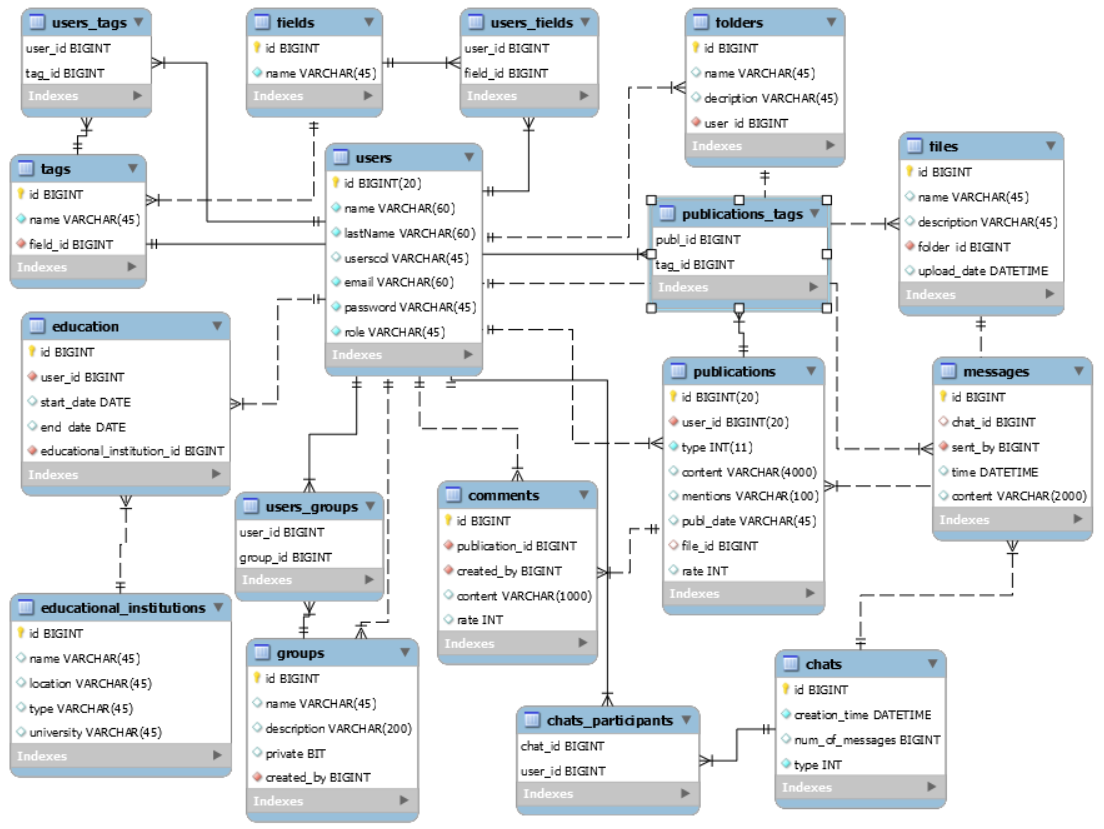
\includegraphics[scale=0.9]{slike/shema.png}}
		\captionof{figure}{EER dijagram}
\end{figure}
